\documentclass[11pt,letterpaper]{article}
\usepackage[margin=0.75in]{geometry}
\usepackage[T1]{fontenc}
\usepackage{lmodern,microtype,amsmath,graphicx}
\usepackage[numbers,sort&compress]{natbib}
\usepackage[colorlinks=true,urlcolor=blue,citecolor=blue,linkcolor=black]{hyperref}
\usepackage{titlesec}
\usepackage{caption}
\usepackage{float}
\titleformat{\section}{\normalsize\bfseries}{}{0pt}{}
\titlespacing*{\section}{0pt}{7pt}{3pt}
\captionsetup{font=small,labelfont=bf,skip=3pt}
\setlength{\parindent}{0pt}
\setlength{\parskip}{3pt}
\setlength{\bibsep}{1pt}
\setlength{\textfloatsep}{8pt}
\setlength{\intextsep}{7pt}
\setlength{\emergencystretch}{2em}
\providecommand{\doi}[1]{\href{https://doi.org/#1}{doi: #1}}
\begin{document}
\begin{center}
{\large\bfseries Predicting Gene-Pair Responses Beyond Additivity\par
with Biological Embeddings and Set Attention\par}
\vspace{3pt}
Pramika Garg \quad | \quad UNI: pg2899 \quad | \quad Interim report
\end{center}
\vspace{-6pt}

\section{Introduction}
Combination therapeutics motivate predicting how target effects combine. Joint gene activation can reinforce or suppress responses and alter differentiation~\cite{norman2019}. I ask whether gene embeddings and attention improve expression prediction for unseen combinations. Ahlmann-Eltze et al. found that adding measured single-gene effects outperformed the tested deep-learning methods~\cite{ahlmann2025}. I therefore treat additivity as the main comparator. This report presents data analysis, five-partition baselines, and cell-level GEARS~\cite{roohani2024} compared with a DepMap-feature and set-attention extension. K562 gene activation supports target-prioritization research, but cannot establish drug efficacy.

\begin{figure}[H]
\centering
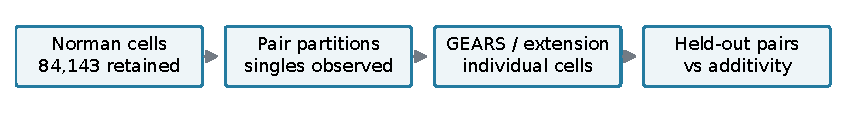
\includegraphics[width=\linewidth]{gpu/figures/01_workflow.pdf}
\caption{Completed interim workflow. Simple baselines use five pair partitions. The two cell-level models share one partition, one initialization and five training epochs.}
\label{fig:workflow}
\end{figure}

\section{Data and exploratory analysis}
I downloaded the scFoundation-processed Norman Perturb-seq AnnData release used in~\cite{ahlmann2025}. It contains 84,986 cells, 19,264 genes and 227 conditions. Excluding two conditions involving \textit{IER5L}, absent from the supplied GO dictionary, removed 843 cells. The retained data contain \textbf{84,143 cells, 100 single-gene conditions, 124 pairs and one control condition}. Control cells number 7,275. Conditions contain 46--7,275 cells, with median 281 (Fig.~\ref{fig:eda}A).

I processed the sparse matrix in chunks and computed condition means, variances and cell-level summaries. The supplied expression values are nonnegative and continuous, with \texttt{log1p} metadata. I used this supplied scale without a second normalization. No stored expression entries were nonfinite, and 85.1\% of matrix entries were zero (Fig.~\ref{fig:eda}B). Principal component analysis (PCA) of condition means on the 1,000 highest-mean control genes explains 35.1\% and 22.6\% of variance in its first two components. Singles and pairs overlap rather than form separate groups (Fig.~\ref{fig:eda}C). Hemoglobin genes \textit{HBZ}, \textit{HBG2} and \textit{HBG1} have the largest absolute PC2 loadings. This PCA describes response variation and is not a model input.

\begin{figure}[H]
\centering
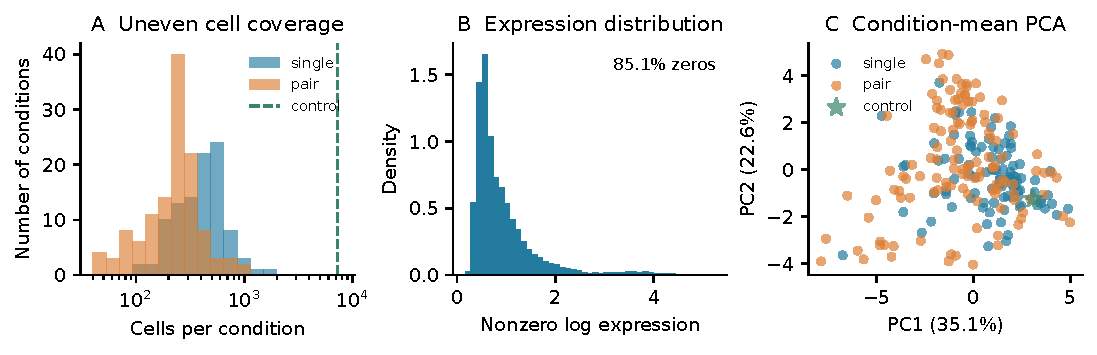
\includegraphics[width=\linewidth]{interim/figures/02_eda.pdf}
\caption{Original exploratory plots. A: cell counts per condition; the dashed line marks control coverage. B: sampled nonzero expression values; the zero fraction uses the full retained matrix. C: centered, unscaled PCA of all 225 condition means, colored by condition type.}
\label{fig:eda}
\end{figure}

\newpage
\section{Methods}
\textbf{Partitions and baselines.} I generated five random pair partitions using seeds 101, 202, 303, 404 and 505. Each contains 62 training, 31 validation and 31 test pairs. All singles and controls remain available for training, and each condition's cells stay together. Across partitions, 155 test appearances cover 98 unique pairs. The additive prediction is $\widehat\mu^{\mathrm{add}}_{AB}=\mu_A+\mu_B-\mu_{\mathrm{ctrl}}$, where each $\mu$ is a condition mean on the supplied expression scale. Other baselines predict the control mean or the equally weighted mean of training perturbation conditions.

Primary evaluation uses mean squared error (MSE) on the same 1,000 genes selected from controls. I calculated paired improvements $D_{p,s}=\mathrm{MSE}_{\mathrm{add},p,s}-\mathrm{MSE}_{\mathrm{model},p,s}$. Positive values favor the model. Repeated held-out results are averaged within each pair before equal-weight summaries. Bootstrap intervals use 10,000 draws of pairs and are conditional on the fitted predictors. Overlapping partitions and shared genes do not provide independent biological replication.

\textbf{Model implementation.} I trained the pinned upstream GEARS class and an extension combining frozen DepMap dependency profiles with permutation-invariant set attention, motivated by MORPH~\cite{he2025}. The labeled \href{https://doi.org/10.6084/m9.figshare.21637199}{DepMap 22Q4} release excludes K562 and its derivative; 96/100 targets have features. Missing targets receive zeros and a presence indicator. A learned projection adds normalized features after the GO encoder; self-attention and learned-seed pooling~\cite{lee2019} replace sum aggregation. Both models use 19,264 readouts, 64 hidden units, the official GO graph (9,853 nodes), and coexpression from individual training singles/control cells only.

Both fits use 67,592 training cells, upstream fourth-power/direction loss, Adam ($10^{-3}$ learning rate, $5\times10^{-4}$ weight decay), batch size 32 and learning-rate halving each epoch. Measured T4 speed selected five epochs each within a shared three-hour allowance. Partition 101, seed 17, FP16 and validation-only checkpoint selection are shared. Condition-mean inference averages the additive control-input path exactly at batch size one. The upstream graph batching behavior is retained; this and the processed release, short budget and validation metric preclude an exact reproduction claim.

\section{Preliminary results}
Across the 98 unique tested pairs, mean MSE is \textbf{0.00929 for additivity}, 0.0206 for the training mean and 0.0364 for no change (Fig.~\ref{fig:results}A). Additivity also has lower mean error in every individual partition. The training-mean predictor's paired improvement is $-0.0113$ (95\% interval $[-0.0139,-0.00872]$), favoring additivity.

On the same 31 test pairs in partition 101, MSE is \textbf{0.01098 for additivity}, 0.01375 for GEARS and 0.01985 for the DepMap/attention extension (Fig.~\ref{fig:results}B). Both finished five epochs; validation selected epoch 3. GEARS outperformed additivity on 7/31 pairs and the extension on 6/31. Paired improvements are $-0.00277$ and $-0.00886$, respectively. The extension did not improve this configuration; changing both prior and aggregation does not isolate either component's effect. Five epochs and one split/seed also limit generalization. Total timed execution was 109 minutes, within the cap.

Separately, splitting cells independently within controls, singles and pairs gives median interaction-residual correlation 0.435 across all 124 pairs. This moderate within-screen repeatability is not independent biological replication.

\begin{figure}[H]
\centering
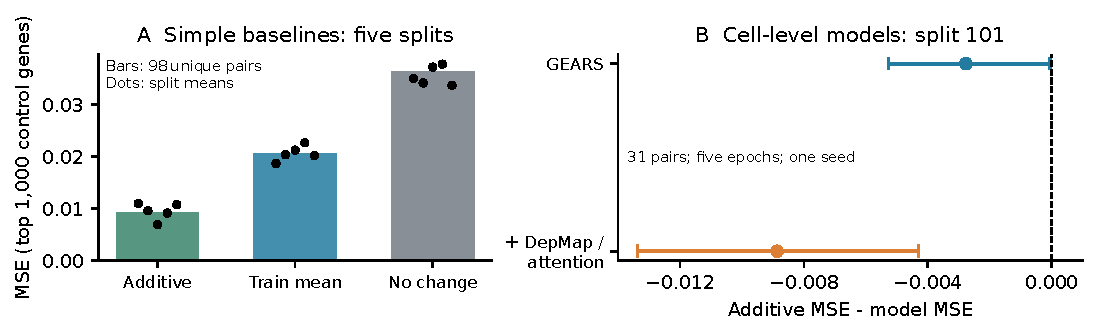
\includegraphics[width=\linewidth]{gpu/figures/03_performance.pdf}
\caption{Measured prediction performance. A: bars average within unique pairs before averaging across pairs; dots show five partition means. B: points show additive-minus-model MSE with 95\% pair-bootstrap intervals on the same 31 test pairs. Negative values favor additivity. Intervals are conditional on these fitted models and do not measure split/seed variability.}
\label{fig:results}
\end{figure}

\section{Next steps}
I will repeat fits across the five partitions and two seeds, evaluate longer schedules, and separate embedding from aggregation effects in the six planned configurations. GenePT~\cite{chen2025} was tested only in earlier condition-mean pilots. I will also examine validation instability and the upstream batch-dependent graph implementation. Sparse combinations, four missing DepMap targets and residual noise limit power. The prespecified final comparison remains attention plus DepMap versus additivity, with validation-only selection. These preliminary negative results do not establish that embeddings cannot help or interactions are absent.

\textbf{Reproducibility.} The accompanying \texttt{interim/} and \texttt{gpu/} folders contain scripts, split lists, measured results, dependency versions and source hashes. Exported predictions independently reproduce every reported scoring subset; artifact hashes, validation selection and elapsed time were checked. The earlier pilots are preserved. Public raw data and large checkpoints are omitted from the small code package.

\bibliographystyle{abbrvnat}
\bibliography{Interim_Report_References}
\end{document}
